% !Mode:: "TeX:UTF-8"                                  %  采用UTF-8编码
\documentclass[a4paper,12pt,hyperref]{ctexart}
\usepackage[text={150mm,240mm},left=20mm,vmarginratio=1:1]{geometry}
\usepackage{hologo}
\newcommand{\BibTeX}{\hologo{BibTeX}}
\usepackage{minted}
\usepackage{cprotect}
\usepackage{marginnote}
\usepackage{graphicx}
\graphicspath{{./figures/}}
\usepackage{natbib}
\hypersetup{pdfstartview=FitH,
            CJKbookmarks=true,
            bookmarksnumbered=true,
            bookmarksopen=true,
            colorlinks=true, %注释掉此项则交叉引用为彩色边框(将colorlinks和pdfborder 同时注释掉)
            pdfborder=001,   %注释掉此项则交叉引用为彩色边框
            citecolor=blue,% magenta, cyan 文献引用的颜色设定
            urlcolor=blue,
            linkcolor=blue,
            linktocpage=true,
            pdfauthor={Marlin, China Jiliang University, <yjccjlu@gmail.com>}
           }

\newcommand{\secref}[1]{第\ref{#1}节}
\newcommand{\rmk}{{\textbf{注:}}}
\newcommand{\cau}{{\textbf{警告:}}}
\newcounter{mycnt}
\setcounter{mycnt}{1}

\title{自然科学引文和参考文献\thanks{本文档适用于natbib宏包8.31b版(2010/09/13).}\\
 \normalsize (作者-年份格式与数字格式)
}
\author{Patrick W. Daly \\ \normalsize 翻译: \href{mailto:yjccjlu@gmail.com}{Marlin}}
\date{2015 年 2 月 14 日}

\begin{document}
\maketitle
\begin{abstract}
  natbib宏包重定义了\LaTeX{}命令\verb|\cite|, 可以采用作者年份格式或者数字格式引用文献,
   适用于plain等标准的参考文献格式,
   也与 harvard, apalike, chicago, astron, authordate以及natbib等兼容。

  与上述宏包相比, natbib宏包不仅支持众多的作者年份格式, 也支持标准的数字格式引用。
  事实上, 它还可以在作者年份的文献格式下产生数字格式引用, 而且很容易在两种引用模式间切换。
  为此, 它也提供了替代标准\LaTeX{}文献格式的专用格式(.bst)。

  narbib宏包可以定义引用格式(如括号以及不同引用条目间标点的类型等),
   甚至可以关联文献格式名以自动激活不同引用格式,
   也可以通过当前的配置文件natbib.cfg为.bst文件定义引用格式。

  natbib宏包与babel, index, citeref, showkeys, chapterbib, hyperref, koma等宏包
   以及amsbook, amsart等文档类兼容,
   也能实现cite宏包的排序与压缩功能, 还能实现Thorsten Ohl写的mcite宏包的多个引用的合并功能。
  然而, natbib宏包本身与cite或mcite宏包不兼容。

  应该注意的是实现文献列表中增加引用页码功能的citeref宏包必须在natbib宏包之后调用。
  (调用hyperref宏包时设定pagebackref选项也有此功能, 而且提供了超链接。)

  此外, natbib宏包为大多常见的参考文献格式提供了统一而灵活的接口。
\end{abstract}
\newpage
\tableofcontents
\newpage

\section{简介}
natbib宏包扩展了\LaTeX{}, 不仅提供数字格式引用,
 也提供作者年份格式引用。
标准\LaTeX{}只允许数字格式引用, 而1993年natbib宏包发布之前,
 所有实现作者年份格式的扩展都局限于此。
因为这些扩展一般都增加了新的命令(natbib宏包也是这样),
 使用了这些命令的文档在扩展编辑后只能用于数字格式引用。

natbib宏包作了调整, 切换作者年份格式与数字格式只需设置一个选项,
 不需要改动源文档。
此宏包现在已经是标准\LaTeX{}安装包的一部分, 符合很多期刊的要求。
同时, 由于它的易用性以及可配置性,
 此宏包已经在众多\LaTeX{}社区作为引用宏包的首选。

跟所有宏包一样, natbib宏包可以附带可选项在导言区调用, 例如%
\begin{minted}[xleftmargin=1cm]{tex}
  \usepackage[sectionbib,square]{natbib}
\end{minted}
可选项sectionbib指明, 当调用宏包chapterbib宏包时,
 参考文献作为一节出现在各章最后(参见\secref{sec2.15})。
可选项square指明参考文献的引用放在一对方括号之内, 而不是放在一对圆括号之内。
调用natbib宏包时可使用的全部选项参见\secref{sec5}.

在文档正文开始处可以指定参考文献格式, 如
\begin{minted}[xleftmargin=1cm]{tex}
  \begin{document}
  \bibliographystyle{plainnat}
\end{minted}
这里plainnat指明参考文献格式, \BibTeX{}程序使用它从参考文献数据库生成实际的参考文献。
plainnat是标准的plain格式(仅限数字格式)在natbib下的对应版本。
别的可用参考文献格式详见\secref{sec2.1}或在\TeX{}系统安装目录查找.bst文件。

命令\verb|\bibliographystyle|可以放置在文档的任何位置,
 但还是建议放在文档开始处, 以便于辨认、修改。

在正文中引用文献,形如
\begin{minted}[xleftmargin=1cm]{tex}
  \citep{jon90} 生成括号引用 (Jones et al., 1990)
  \citet{jon90} 生成文本引用 Jones et al. (1990)
\end{minted}
这里\verb|\citep|和\verb|\citet|并不是\LaTeX{}的标准命令,而是natbib宏包定义的专用命令。
\LaTeX{}标准命令\verb|\cite|应尽量避免使用,因为natbib宏包重定义了此命令,
 使它在作者年份格式下等同于\verb|\citet|,在数字格式下等同于\verb|\citep|。
natbib宏包还定义了很多其他命令产生一些特别的效果(参见\secref{sec2.4})。

上述例子中的jon90是文献的引用标签,在\BibTeX{}文献数据库中定义,
 或者在thebibliography环境中定义(参见\secref{sec2.2}),如
\begin{minted}[xleftmargin=1cm]{tex}
  \begin{thebibliography}{1}
    \bibitem[Jones et al.(1990)]{jon90}
    . . . . .
  \end{thebibliography}
\end{minted}
此环境生成真正的参考文献,\verb|\bibitem|命令将文献条目与引用通过引用标签关联起来,
 这里的jon90就是引用标签。
引用标签可以任意指定,只要不重复即可。
方括号中内容为文献的引用信息,作者为Jones et al.,年份为1990。
注意这两部分内容根据引用命令能以不同的方式结合在一起。
事实上,如果使用了数字格式的引用,方括号中的引用信息会被忽略,只有顺序数字作为引用。

thebibliography环境可以手工书写,但更好更安全的方式是由\BibTeX{}来生成。
为此,我们需要使用前文提到的\verb|\bibliographystyle|命令,以及在文档末尾放置
\begin{minted}[xleftmargin=1cm]{tex}
  \bibliography{mybib}
  \end{document}
\end{minted}
这里mybib是\BibTeX{}文献数据库名,后缀为.bib。
mybib.bib中包含了文档中引用到的文献的相关信息。

本文档其余部分介绍了natbib宏包可能的全部细节。


\section{如何使用本宏包}
本文中,我们区分了引用模式(引用文献时的标点类型等)与引用格式(作者年份格式与数字格式)。
引用模式不同于参考文献格式,并不是在.bst文件中指定。

\subsection{新的参考文献格式}\label{sec2.1}
natbib宏包提供了三种文献格式.bst文件来代替标准\LaTeX{}数字格式:
\begin{minted}[xleftmargin=1cm]{tex}
  plainnat.bst     abbrvnat.bst     unsrtnat.bst
\end{minted}
它们可以用来生成与相应标准格式风格相同的文献列表,但更适于natbib宏包。
其优势在于它们在数字格式与作者年份格式下都可以使用。

这些.bst文件并没有穷尽所有格式,还有很多适于natbib宏包的格式。
当然也可以使用本宏包作者提供的custom-bib程序(称为makebst)生成自己的.bst格式文件。

\subsection{thebibliography的语法}\label{sec2.2}
thebibliography环境中的\verb|\bibitem|命令提供所引用文献的作者姓名及年份等信息。
natbib宏包希望这些信息能以上面提到的格式文件.bst指定的样式呈现出来。
(也可以由早期的Harvard和Chicago等宏包使用。)
如果不使用\BibTeX{},就必须自己设定thebibliography环境,使它符合natbib宏包要求。

需要使用如下形式的语法:
\begin{minted}[xleftmargin=1cm]{tex}
  \bibitem[Jones et al.(1990)]{jon90}...
\end{minted}
或者
\begin{minted}[xleftmargin=1cm]{tex}
  \bibitem[Jones et al.(1990)Jones, Baker, and Williams]{jon90}...
\end{minted}
方括号中的内容包含了引用信息,缩略作者列表Jones et al.,年份1990,
 可选的完整作者列表Jones, Baker, and Williams。
如果省略完整作者列表,则用缩略作者列表代替。
将年份括起来的括号并不是引用信息必须的,只是用来界定作者列表与年份。
即使在引用模式中使用方括号,这里也必须使用圆括号。
在年份括号前后不能有空格,否则它将被看成是作者列表的一部分。

\rmk 如果某一条\verb|\bibitem|条目不符合natbib的语法,将被强制转换成数字格式,
 因为此时natbib宏包无法确定作者与年份信息。

\subsection{基本的引用命令}\label{sec2.3}
natbib宏包也可以与为别的宏包甚至陈旧的宏包如Harvard等设计的文献格式配合使用。
然而,这里与下节介绍的命令是由natbib宏包定义的,也可以由其他文献格式使用。
\cprotect\marginnote{\verb|\citet|\\\verb|\citep|}

natbib宏包提供了两个基本的引用命令,
 \verb|\citet|与\verb|\citep|分别实现文本引用与括号引用。
还提供了带*的版本,\verb|\citet*|与\verb|\citep*|,区别在于生成完整的作者列表,而不是缩略作者列表。
这些命令都可以通过可选参数在文献引用标记前后增加说明信息。
\begin{center}
  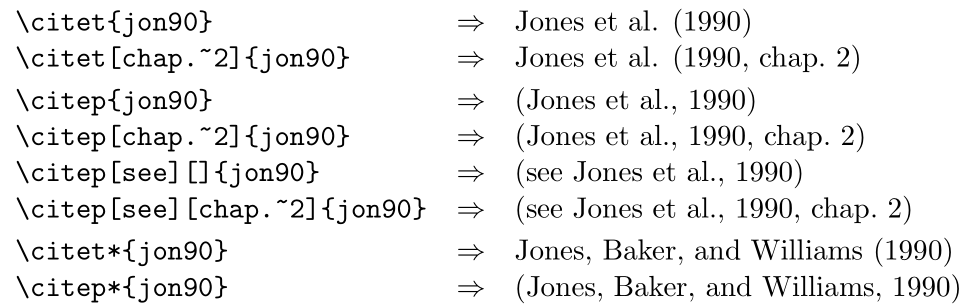
\includegraphics[width=.85\textwidth]{natbib1}
\end{center}
带*的版本只能在.bst格式支持的情况下生成完整作者列表,否则生成缩略作者列表。

在标准\LaTeX{}中,\verb|\cite|命令只能有一个可选参数提供引用标记后的说明信息,
 这里一个可选参数提供引用标记后的说明信息,
 两个可选参数分别提供引用标记前和引用标记后的说明信息。
如果只需要引用标记前的说明信息,像上述例子那样,必须提供一个对应引用标记后信息的空的可选参数。

更复杂的文本与引用的混合使用可以由用途更多的\verb|\citetext|命令实现,参见\secref{sec2.4}。

多个引用可以由一个\verb|\cite|命令使用多个引用标签实现.
如果相邻的引用文献有相同的作者但年份不同,则作者信息不会重复出现。
\begin{center}
  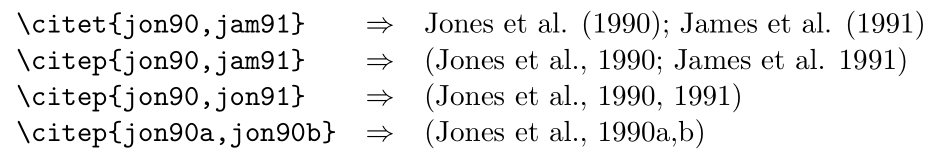
\includegraphics[width=.85\textwidth]{natbib2}
\end{center}

这些例子是针对作者年份格式的,如果是数字格式,结果将是:
\begin{center}
  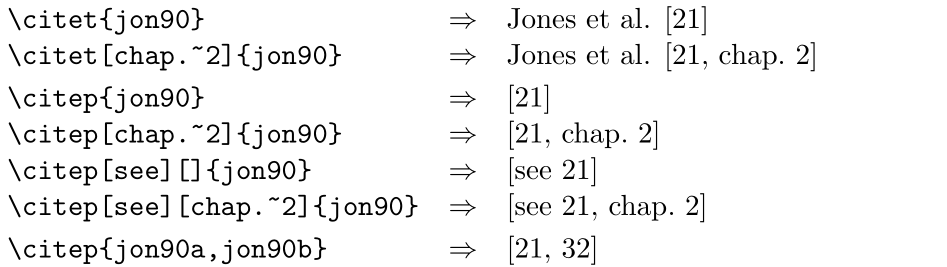
\includegraphics[width=.85\textwidth]{natbib3}
\end{center}
只有.bst文件支持作者年份格式,作者信息才会显示。
标准的.bst文件如plain.bst只支持数字格式,不会将作者年份信息传递给\LaTeX{}。
这种情况下,\verb|\citet|将生成形如“(author?) [21]”的引用标记。

在natbib的早期版本中,\verb|\cite|命令可以用于文本或括号引用,\cprotect\marginnote{\verb|\cite|}
 放在方括号中的内容表示插入说明信息。
出于兼容性考虑,保留了这种用法,但不再提倡这么用。

因为不带说明信息的\verb|\cite|命令在作者年份格式下相当于\verb|\citet|,
 在数字格式下相当于\verb|\citep|。
带*的版本以及带一个或两个说明信息的命令,也是类似使用。

有时候需要多条引用信息按照参考文献列表的中的顺序排列,而不是按照\verb|\cite|参数中的排列顺序。
宏包选项sort实现此功能。
详情参见\secref{sec2.16}。

有些出版机构要求所有文献在第一次被引用时给出全部作者列表,之后的引用只需给出缩略作者列表。
调用natbib宏包时加longnamesfirst选项即可实现此功能。
详情参见\secref{sec2.18}。

\subsection{扩展的引用命令}\label{sec2.4}
引用的另一种形式,\cprotect\marginnote{\verb|\citealt|\\\verb|\citealp|}
 \verb|\citealt|命令与\verb|\citet|命令的差别只在于引用标记中没有括号。
类似地,\verb|\citealp|命令是\verb|\citep|命令没有括号的版本。

\cprotect\marginnote{\verb|\citenum|}\verb|\citenum|命令生成数字编号引用,即使在作者年份格式下,
 但不产生括号,也不会生成上标形式。
这样设计是为了更容易的以普通文本的方式对引用编号进行引用。

除了\verb|\citenum|之外,这些命令也可以一次引用多条引文献,添加说明信息,以及带*版本等用法。
\begin{center}
  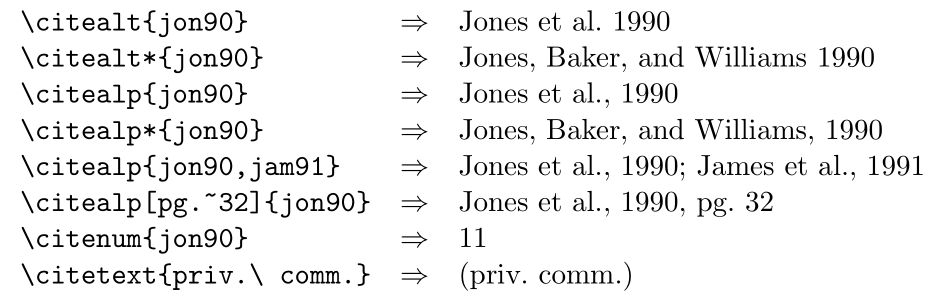
\includegraphics[width=.85\textwidth]{natbib4}
\end{center}

\cprotect\marginnote{\verb|\citetext|}\verb|\citetext|命令可以在当前引用标记括号内插入任意文本内容。
此命令经常与\verb|\citealp|命令配合使用。
例如:
\begin{minted}[xleftmargin=1cm]{tex}
  \citetext{see \citealp{jon90}, or even better \citealp{jam91}}
\end{minted}
生成如下形式的引用:
\begin{minted}[xleftmargin=1cm]{tex}
 (see Jones et al., 1990, or even better James et al., 1991).
\end{minted}

\cprotect\marginnote{\verb|\citeauthor|\\\verb|\citeyear|\\\verb|\citeyearpar|\\\verb|\citefullauthor|}

在作者年份格式下,有时候只需要引用作者而不需要引用年份,或者是只需要年份而不需要作者。
此宏包提供了一系列扩展的引用命令。
\begin{center}
  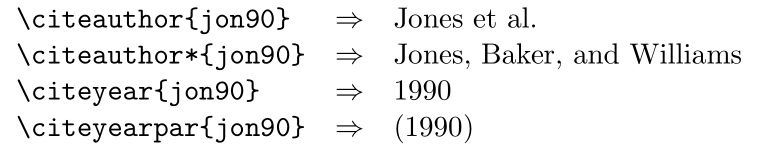
\includegraphics[width=.65\textwidth]{natbib5}
\end{center}
这里的\verb|\citefullauthor|命令等价于\verb|\citeauthor*|命令。

如果文献条目中缺少完整的作者列表,\verb|\citeauthor*|命令等同于\verb|\citeauthor|命令,
 只生成缩略作者列表。
这种情形也适用于\verb|\citet|命令\verb|\citep|命令。

跟使用标准\LaTeX{}格式文件.bst一样,如果文献条目中缺少作者或者年份信息,
 这些命令会产生警告信息。

\rmk 即使使用了作者年份格式.bst,这些命令也可以用于数字模式引用。

\rmk 这些\verb|\cite..|命令有相同的语法,允许多条文献引用,
 可以有附加说明信息(\verb|\citeyear|和\verb|\citenum|命令没有带*版本的用法)。
为\verb|\citeyear|和\verb|\citeauthor|命令添加说明信息没有实际意义,尤其是多条文献引用时,
 但是可以这么使用,也不会报错,只是显示结果会有些奇怪而已。
例如,在数字引用模式下,这些说明信息完全被忽略;
 在作者年份引用模式下,只接受引用标记后的说明信息。
也不推荐在\verb|\citet|命令中引用多条文献(在我看来这没有什么意义),
 如果这么用了,而且添加了说明信息,引用标记前的说明信息会出现在每一个年份前,
 而引用标记后的说明信息只出现在最后一个年份后。
这些都是显而易见的问题,但没必要为了解决不合理的使用造成的问题而花费太多精力。

总的来说,只提倡在\verb|\citep|命令中使用附加说明信息,
 但是也可以在作者年份引用模式下,在\verb|\citet|命令引用单条文献时使用附加说明信息。
在别的情形下使用附加说明信息会产生不可预期的结果。

\subsection{强制姓名大写}\label{sec2.5}
如果首作者的姓名中含有\textsl{von}部分,例如“della Robbia”,
 即使在句首,\verb|\citet{dRob98}|也只能产生形如“della Robbia (1998)”的引用。
此时,我们可以使用\verb|\Citet|命令强制首字母大写。
还有一些其他的强制首字母大写的命令。
\begin{center}
  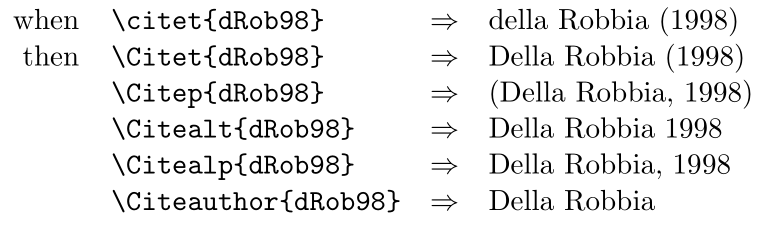
\includegraphics[width=.85\textwidth]{natbib6}
\end{center}
这些命令也都有相应的显示完整作者列表的带*版本的用法。

\rmk 实现首字母大写命令的写法有些讨巧,可以作用于写在\verb|\bibitem|文献条目中作者信息,
 甚至使用了旧的字体设置命令也可以使用,但是\LaTeXe{}字体设置命令会产生冲突。
例如
\begin{center}
  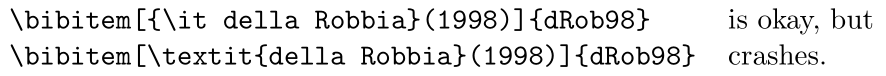
\includegraphics[width=.85\textwidth]{natbib7}
\end{center}

\subsection{引用别名}\label{sec2.6}
\cprotect\marginnote{\verb|\citetalias|\\[-13mm]\verb|\defcitealias|\\[5mm]\verb|\citepalias|}
有时候我们希望通过某个特殊的名称来引用文献,而不是作者信息等方式,
 如“Paper \Roman{mycnt}”、\stepcounter{mycnt}“Paper \Roman{mycnt}”等。
可以定义并使用这些别名,不论是文本引用还是括号引用,例如:
\begin{center}
  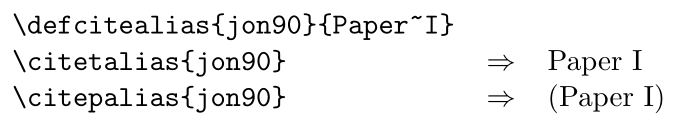
\includegraphics[width=.8\textwidth]{natbib8}
\end{center}
这些命令的使用类似于\verb|\citet|和\verb|\citep|,
 可以在参数中引用多条文献,可以包含附加说明信息,可以标记为超链接,等等。

如果在定义之前就使用了别名,或者重定义一个已经使用了的别名,会产生警告信息。
如果给一个不存在的文献条目定义别名,并不会产生警告信息,直到此别名被使用时才会产生警告信息!

\secref{sec2.7}给出了通过代码名称引用的方法。

\subsection{缺少作者和年份信息的文献}\label{sec2.7}
对于没有作者信息的文献如何引用?
这是困扰了我很久的一个问题,但现在我有了解决办法。
在标准的\BibTeX{}格式中,当作者或编者信息缺失时,
 在文献条目中使用一个称为“KEY”的域来按字母顺序排序。
在作者年份格式中,更进一步将“KEY”域插入到作者信息的位置。
我们可以想象此时为文献指定了代码名称。
例如
\begin{minted}[xleftmargin=1cm]{tex}
 @MANUAL{handbk98,
   title = {Assembling Computers},
   year = 1998,
   organization = {MacroHard Inc.},
   key = "MH-MAN"
 }
\end{minted}
使用plain文献格式时,key的值“MH-MAN”只是用于文献列表中对文献排序;
 使用plainnat或别的作者年份文献格式时,ket的值被直接用于作者信息。
我们可以通过\verb|\citeauthor{handbk98}|引用此文献得到MH-MAN,
 或者通过\verb|\citetext{\citeauthor{handbk98}}|得到括号引用(MH-MAN)。

如果参考文献格式将文献条目里可选项中的日期信息留空,
 natbib宏包处理起来更简单,例如
\begin{minted}[xleftmargin=1cm]{tex}
  \bibitem[MH-MAN()]{handbk98}
\end{minted}
引用标记中会取消日期,标点以及括号,就像\verb|\citet|命令的效果一样。
这意味着natbib宏包会像上面的例子那样,
 自动匹配\verb|\citet|或\verb|\citep|的格式。
而文献列表中的文献条目中仍然会显示日期信息。

当缺失的作者或编者信息由key域的值替换后,
 natbib宏包根据省略了日期信息的文献条目对文献格式做了相应修改。

类似地,如果年份信息缺失,在文献条目中也会将年份域留空,
 引用这样的文献将只生成作者姓名。

\rmk 这种情形有各种可能的处理。
比如可以将引用代码放置到文献条目的作者位置,将年份域留空,
 然后像alpha格式(字母顺序排列)那样生成引用。
第二组代码(甚至就是作者姓名)放置到一般情况下完整作者姓名列表出现的位置,
 以便\verb|\cite*|命令使用。
例如
\begin{minted}[xleftmargin=1cm]{tex}
  \bibitem[MH-MAN()MacroHard Inc.]{handbk98}
\end{minted}

\subsection{plainnat系列格式的扩展}\label{sec2.8}
\secref{sec2.1}中提到的natbib宏包特有的.bst格式文件与标准的格式相比,
 有一些扩展的域:
\begin{description}
  \item[ISBN] 为书籍类文献添加ISBN号
  \item[ISSN] 为期刊类文献添加ISSN号
  \item[URL] 为在线文献添加网址链接
  \item[DOI] 现在很多期刊采用的比URL更可靠的数字对象标识符
  \item[EID] 在线期刊和纸质期刊用来代替页码的电子身份证,也用作期刊的序列号
\end{description}

DOI和URL往往都比较长,这会导致难看的断行或者突出到页边界。
这个问题可以通过调用Donald Arseneau编写的url宏包解决,
 此宏包允许文本在不带连字符的标点处断行。
该宏包的调用可由natbib宏包自动检测到,并重定义一些适当的命令。
URL显示为打字机字体,DOI显示为罗马字体。
如果没有调用url宏包,URL和DOI这些内容将不会自动断行。

像\secref{sec2.7}提到的那样,plainnat格式和plain格式对key域的值采用不同的处理方式。
plain格式下,只是将key域的值用于没有作者信息时对文献字母顺序排序。
plainnat格式下,将key域的值实际插入到文献信息与引用标记的作者位置。
进一步,如果文献条目中年份信息也留空,
 \verb|\citep|命令只能生成“作者”内容,
 此时即显示key域的值。
这应该是为此文献设定的代码。

\subsection{引文输出格式的选择}\label{sec2.9}
\cprotect\marginnote{\verb|\setcitestyle|}
上面的例子显示了默认的引用风格的样式。
不论是数字格式还是作者年份格式,这些样式都可以通过\verb|\setcitestyle|命令改变。
此命令采用一组逗号分隔的关键词作为参数。
(这个命令是版本8以上的natbib宏包新增加的。)
\begin{itemize}
  \item 引用模式:authoryear(作者年份格式)、numbers(数字格式)、
       super(数字上标格式)。(对应于\verb|\bibpunct|命令的第四个参数)
  \item 括号:round(圆括号)、 square(方括号)、 open=\{左括号\}和
       close=\{右括号\}。(对应于\verb|\bibpunct|命令的第一和第二个参数)
  \item 引用标记间的分隔符:semicolon(分号)、comma(逗号)、citesep=\{分隔符\}。
       (对应于\verb|\bibpunct|命令的第三个参数)
  \item 作者与年份间的分隔符:aysep=\{分隔符\}。(对应于\verb|\bibpunct|命令的第五个参数)
  \item 同一个作者不同年份间的分隔符:yysep=\{分隔符\}。(对应于\verb|\bibpunct|命令的第六个参数)
  \item 引用命令可选参数说明信息前的分隔符:notesep=\{分隔符\}。(对应于 \verb|\bibpunct| 命令的可选参数)
\end{itemize}
默认设置相当于:
\begin{minted}[xleftmargin=0cm]{tex}
  \setcitestyle{authoryear,round,comma,aysep={;},yysep={,},notesep={, }}
\end{minted}

例1,在作者年份格式下,
\begin{minted}[xleftmargin=0cm]{tex}
  \setcitestyle{square,aysep={},yysep={;}}
  \citep{jon90,jon91,jam92}
\end{minted}
将生成[Jones et al. 1990; 1991, James et al. 1992]形式的引用。

例2,在作者年份格式下,
\begin{minted}[xleftmargin=1cm]{tex}
  \setcitestyle{notesep={; },round,aysep={},yysep={;}}
  \citep[and references therein]{jon90}
\end{minted}
将生成 (Jones et al. 1990; and references therein)形式的引用。

\rmk
\begin{itemize}
  \item 没有指明修改的参数保持不变;
  \item 参数的次序无关紧要;
  \item 作者与年份间的分隔符只用于作者年份格式的引用,数字格式下无效;
  \item 不同年份间的分割用于一次性引用的多条文献有相同作者的情形,而且总会插入一个空格;
      如果年份也相同,则生成形如 ‘2007a,b’的引用,此时不会插入空格;如果希望此时插入空格,
      参数可以设置为\verb|yysep={,~}|;
  \item 在数字格式下,相同作者多条文献的引用,例如\verb|\citet{jon90,jon91}|会生成形如
       ‘Jones et al. [21, 22]’的引用,数字间插入标点;而且自动加入空格,但在数字上标格式下不加入空格;
  \item 除逗号外,单个符号不需要放在\{\,\}内,例如,yysep=;是可以接受的参数。
\end{itemize}%
\cprotect\marginnote{\verb|\bibpunct|}

原有的设置引用格式的命令是\verb|\bibpunct|,此命令带有六个必选参数与一个可选参数:
\begin{enumerate}
  \item 引用标记的左括号,默认是(
  \item 引用标记的右括号,默认是)
  \item 多条引用间的分隔符,默认是;
  \item 字母n代表数字格式,字母s代表数字上标格式,别的字母代表作者年份格式,默认是作者年份格式
  \item 作者与年份之间的分隔符
  \item 相同作者的文献连续引用时,年份或数字之间的分隔符,默认是,
\end{enumerate}

可选参数是说明信息前的符号,默认是逗号加一个空格。
如果重定义了分隔符,需要其后的空格的话,必须显式指定。

上述\verb|\setcitestyle|命令的两个例子,可以由如下命令分别实现:
\begin{minted}[xleftmargin=1cm]{tex}
  \bibpunct{[}{]}{,}{a}{}{;}
  \bibpunct[,~]{(}{)}{,}{a}{}{;}
\end{minted}

\subsection{预定义引用格式}\label{sec2.10}
\cprotect\marginnote{\verb|\citestyle{name}|\\\verb|\bibstyle@name|}
如果要经常使用一种特定的引用记号,可以将这些记号放置在当前的配置文件natbib.cfg中,
 然后通过\verb|\citestyle{name}|命令调用。
这里name是通过\verb|\bibstyle@name|命令为想要使用的引用记号定义的名称。

例如,美国地球物理学会(American Geophysical Union,AGU)旗下出版物要求引用标记使用方括号,用分号分隔。
有专门的agu.bst完成大部分格式的设置,但没有包括这些引用标记的要求。
natbib宏包有如下定义以及相应的命令
\begin{minted}[xleftmargin=1cm]{tex}
  \newcommand{\bibstyle@agu}{\bibpunct{[}{]}{;}{a}{,}{,~}}
  \citestyle{agu}
\end{minted}
来实现这些要求。

这样预定义引用风格的方法特别之处在于:
 natbib宏包在文档开始处调用参考文献格式名称来执行\verb|\citestyle|,
 就像使用\verb|\bibliographystyle|命令一样(储存在辅助文件.aux中)。
这意味着引用风格可以直接与参考文献格式.bst文件关联。
这种实现方式可以由指定的文献格式立即改写引用风格,
 就像使用了宏包参数或\verb|\setcitestyle|,\verb|\bibpunct|,\verb|\citestyle|等命令一样。

natbib宏包为以下文献格式预定义了引用风格:
\begin{description}
  \item[plain等4种标准格式:] 方括号,数字格式,逗号分隔
  \item[plainnat等格式:] 方括号,作者年份格式,逗号分隔
  \item[agu(美国地球物理学会):] 方括号,作者年份格式,分号分隔
  \item[egu(欧洲地球科学学会):] 圆括号,作者年份格式,逗号分隔
  \item[agms, dcu, kluwer(Harvard系列):] 圆括号,作者年份格式
  \item[cospar(太空研究委员会):] 斜线,数字格式,逗号分隔
  \item[nature(自然期刊):] 上标
\end{description}
还有很多出于我个人便利考虑的设置。上面列出了大多数主要的改变,可以满足各种一般要求。
可以将这些定义放到当前的配置文件natbib.cfg实现与别的参考文献格式的自动关联。

注意plain和plainnat的预定义中指定了方括号,从而改变了natbib宏包默认的圆括号。

除了\verb|\bibpunct|和\verb|\setcitestyle|命令外,还有很多定义引用风格的方法。
一些数字格式的引用模式常希望有更多的改变,
 有时会要求文献列表中只生成数字而没有常规的方括号。
为适应这样的要求,natbib宏包可以这样定义风格:
\begin{minted}[xleftmargin=1cm]{tex}
  \newcommand{\bibstyle@nature}%
      {\bibpunct{}{}{,}{s}{}{\textsuperscript{,}}%
       \renewcommand\bibnumfmt[1]{##1.}}
\end{minted}
重定义的\verb|\bibnumfmt|命令指明了文献列表中文献数字编号的显示格式。

\subsection{格式命令的优先权}\label{sec2.11}
引用风格(标点以及引用模式)可以由\verb|\setcitestyle|,\verb|\bibpunct|,\verb|\citestyle|等命令
 以及通过\verb|\bibliographystyle{bst}|调用预定义的\verb|\bibstyle@bst|等方式来指定。
还可以通过调用natbib宏包时指定可选参数来实现,\secref{sec5}。
如果同时有几种相冲突的选择会发生什么呢?

\verb|\bibliographystyle|命令具有最低的优先级,因为这种设定引用风格方式对用户并不透明。
接下来是宏包调用时指定可选参数的方法。
最后是\verb|\setcitestyle|,\verb|\bibpunct|,\verb|\citestyle|等命令,
 可以改变其他方式指定的风格。

\subsection{其他的格式选项}\label{sec2.12}
参考文献列表通常以\verb|\section*|或\verb|\chapter*|的形式出现,
 取决于文档所使用的类型。\cprotect\marginnote{\verb|\bibsection|}
如果想设定自己特定的标题,比如要改成带编号的\verb|\section|形式,
 可以由用户自行重定义\verb|\bibsection|来实现。
\cprotect\marginnote{\verb|\bibpreamble|}

\verb|\bibpreamble|命令指定对文献列表的说明信息,其内容会在文献列表标题之后,列表之前插入。
\cprotect\marginnote{\verb|\bibfont|}
这些内容通常以正文字体显示,除非在此命令参数中设定特定字体。
\verb|\bibfont|命令设定整个文献列表的总体字体,但不设定列表前说明信息的字体。

参考文献列表通常采用与正文相同的字体尺寸与风格。
然而,可以通过重定义\verb|\bibfont|来设定文献列表中说明信息后的字体。
例如
\begin{minted}[xleftmargin=1cm]{tex}
  \renewcommand{\bibfont}{\small}
\end{minted}
\cprotect\marginnote{\verb|\citenumfont|}

数字格式引用时编号可以使用不同的字体。
重定义\verb|\citenumfont|可以声明字体如\verb|\itshape|,
 也可以用带参数的命令如\verb|\textit|。
\begin{minted}[xleftmargin=1cm]{tex}
  \renewcommand{\citenumfont}[1]{\textit{#1}}
\end{minted}
上例中的用法优于使用\verb|\itshape|,因为它可以自动进行斜体校正。
\cprotect\marginnote{\verb|\bibnumfmt|}

参考文献列表中数字编号的格式可以由重定义\verb|\bibnumfmt|命令来设定。
例如
\begin{minted}[xleftmargin=1cm]{tex}
  \renewcommand{\bibnumfmt}[1]{\textbf{#1}:}
\end{minted}
将默认的数字编号格式[32]改成粗体不带方括号的编号\textbf{32}:。


作者年份格式的文献列表通常采用悬挂缩进的格式:
 每条文献条目的第一行左对齐,其余行设置距离页边界一定的缩进量。
\cprotect\marginnote{\verb|\bibhang|}
此缩进量默认为1em,可以通过\verb|\setlength|命令
 重定义\verb|\bibhang|的值来进行调整。

\cprotect\marginnote{\verb|\bibsep|}
不论是作者年份格式还是数字格式,
 参考文献列表中文献条目之间的行间距由\verb|\bibsep|的值确定。
如果此值设成0pt,则文献条目间没有额外行间距。
其默认值取决于文档类设定的字体尺寸,基本上就是一条空行。
可以通过\verb|\setlength|命令重定义\verb|\bibsep|的值来进行调整。

\subsection{引用的自动索引}\label{sec2.13}
\cprotect\marginnote{\verb|\citeindextrue|\\\verb|\citeindexfalse|}
如果要文献引用放到索引文件.idx中,
 只需要将\verb|\citeindextrue|命令写在文档任意位置即可。
之后所有的\verb|\cite|命令及延伸命令都会将相应条目插入索引文件。
写上\verb|\citeindexfalse|命令,则相应条目不再插入索引文件。

thebibliography环境中的文献条目命令\verb|\bibitem|也会产生索引条目。
如果不希望产生索引,只需将 \verb|\citeindexfalse| 命令放置到
 \verb|\bibliography| 或 \verb|\begin{thebibliography}| 之前即可。

当然了,跟通常用法一样,
 必须在导言区写上\verb|\makeindex|命令才会激活索引功能。
否则,不会生成任何索引。

要正常生成索引,在运行makeindex之前,
 需确保运行\BibTeX{}后编译文档两次以上。
\cprotect\marginnote{\verb|\NAT@idxtxt|}

索引条目的样式由内部命令\verb|\NAT@idxtxt|设置,
 如果要更改样式,可以在当前配置文件natbib.cfg中重定义此命令。
默认情况下,索引形式为当前括号形式与引用模式下,
 将缩略作者列表或文献编号数字写入括号内。

natbib宏包也可以与David M. Jones编写的index宏包一起使用。
两个宏包的调用次序没有影响。

在index宏包中,可以由\verb|\newindex|命令生成多个索引列表。
例如,可以将所有文献引用索引放到单独的一个索引列表内。
首先,这样的列表需要类似于如下形式的初始化:
\begin{minted}[xleftmargin=1cm]{tex}
  \newindex{cite}{ctx}{cnd}{List of Citations}
\end{minted}
然后,使用natbib宏包中的如下命令将自动引用索引关联到此索引列表:
\begin{minted}[xleftmargin=1cm]{tex}
  \renewcommand{\citeindextype}{cite}
\end{minted}
详情参见index.sty宏包文档。

\subsection{与Hyper\TeX{}的兼容性}\label{sec2.14}
natbib宏包与Sebastian Rahtz 和 Heiko Oberdiek编写的hyperref宏包兼容,
 可用于\LaTeX{}$\to$HTML转换,pdf\TeX{},pdfmark等的实现。
兼容是共有的性质,涉及两个宏包的编码及相互配合方面。

hyperref宏包有个特殊的选项breaklinks,允许链接文本自动断行到下一行,
 避免产生行溢出信息。
默认情况下,链接文本是被限制在一行内的。
对数字格式引用没有问题,但是作者年份格式引用常常会有较长的引用文本,
 容易产生行溢出问题。

\subsection{一个文档内有多个参考文献}\label{sec2.15}
natbib宏包与Donald Arseneau和Niel Kempson编写的chapterbib宏包兼容,
 该宏包允许在一个文档内有多个独立的参考文献列表。
通常用法是一本书的各章有独立的参考文献列表,
 尤其是在各章由不同作者独立编写时。

chapterbib宏包使各章作者可以一种很自然的方式使用参考文献,
 只有将各章汇集在一本书里的作者或编者才需要一些额外的工作。

宏包使用\verb|\include|命令,每个被包含进来的文件有自己的参考文献。
对大规模的书籍,这样的处理有很大的优势。

回顾\verb|\iclude|命令的使用,主文档形如:
\begin{minted}[xleftmargin=1cm]{tex}
  \documentclass{...}
  \includeonly{ch2}
  \begin{document}
    \include{ch1}
    \include{ch2}
    \include{ch3}
  \end{document}
\end{minted}
只导入 ch2.tex 文件,即 ch1.tex 和 ch2.tex 都存在。
如果以前曾经完整地编译过整个文档,那么原来的所有计数器,
 特别是页码、章节编号、交叉引用等任然会保留为前一次编译的效果。
这里的诀窍是每一个被包含进来的文件有自己单独的辅助 .aux文件,
 其中包含了这些信息,即使相应的 .tex文件没有被导入,
 每次编译时这些辅助文件也会被调用。
辅助 .aux文件中也包含了\BibTeX{}使用的引用信息,
 同样会被chapterbib宏包使用。

如果在导言区调用了chapterbib宏包(\verb|\usepackage{chapterbib}|),
 每一个\verb|\cite|命令或\verb|bibitem|命令中的引用标签会关联到当前导入的文件,
 与其他文件中相同的引用标签区别开来。
每一个这样被包含进来的文件必须包含自己的
 \verb|\bibliography| 和 \verb|\bibliographystyle| 命令。
在使用\LaTeX{}编译文档(至少两次)之前,
 要用\BibTeX{}分别编译各个子文档。

\subsubsection{为natbib和chapterbib的特殊考虑}\label{sec2.15.1}
调用chapterbib和natbib宏包的次序是无关紧要的。

chapterbib宏包提供了一个选项sectionbib,
 可以在每章都有自己的参考文献时,
 使参考文献列表以\verb|\section*|的格式替代\verb|\chapter*|的格式排版。
当natbib宏包也被调用时,该选项不起作用了,
 相应地,natbib宏包提供了这一选项来实现此功能。
(调用natbib宏包时总是可以使用sectionbib选项,
 但它只在文档类是book或者report以及它们的扩展类型时才有效。)

如果每一个被导入的子文档要显示自己的参考文献列表,
 就必须包含自己的\verb|\bibliography|命令。
当然,各子文档的这条命令调用的文献数据库可以不同。
然而,特别之处在于每个子文档必须包含自己的\verb|\bibliographystyle|命令,
 各子文档的这条命令还可以指定不同的文献格式。

natbib宏包8.0以上版本中,各章可以有不同的引用风格和模式(作者年份格式或数字格式)。
\verb|\setcitestyle|,\verb|bibpunct|,\verb|\citestyle|等命令可以在文档任何位置指定,
 尤其是在各章的子文档中。
(这是唯一需要指明的地方。)

\subsection{数字格式引用的排序与压缩}\label{sec2.16}
另一个由 Donald Arseneau 编写的宏包cite.sty也改写了数字格式引用文献时的标点以及模式,
 它的所有功能都可以由natbib宏包实现。
然而,它也可以实现数字格式引用标记的排序和压缩,这是很多期刊要求的格式。

当一条引用命令中引用多条文献条目时,引用标记的正常顺序就是引用条目时的顺序。
这通常会生成较长的引用标记列表,形如 [4,2,8,3]。
调用了cite宏包后,会显示为 [2–4,8]。

使cite宏包与natbib宏包兼容是不可能的,因为它们都改写了原始的\verb|\cite|命令。
相应地,我参考了cite宏包的某些代码,使它可用于natbib宏包。
这些代码可以在调用natbib宏包时使用sort或者sort\&compress选项激活其功能。

在作者年份格式下,
 sort选项使\verb|\citet|或\verb|\citep|命令中的引用标记按文献列表中的顺序排版。
通常按姓名的字母顺序,然后是年份顺序。
这样可以避免生成形如 “James et al. (1994b,a)” 的引用标记。
在作者年份格式下,选项sort\&compress等同于sort。

\subsection{数字格式文献的合并}\label{sec2.17}
\begin{minipage}{0.9\textwidth}
  \rmk 合并数字格式文献的代码是 Arthur Ogawa 为美国物理学会设计的。
\end{minipage}

Thorsten Ohl编写的mcite宏包不能跟natbib宏包一起使用。
实现文献合并功能,需要在调用natbib宏包时使用merge选项。

使用merge选项,可以把\verb|\citep|引用的几个不同文献放在文献列表中的同一项,
 为此需要使用*指明主要的和次要的文献。
例如,\verb|\citep{feynmann,*salam,*epr}|生成一个引用标记,
 三篇文献在文献列表中被列在一条文献条目下,共用一个文献编号。

Thorsten Ohl 编写的mcite宏包的一个限制被突破:
 *可以用于任何引用标签。
此宏包语法方面的限制也不再适用。

另一个特色是文献条目中可以插入说明信息:
 在\verb|\citep|命令的参数中,可以在引用标签前加两个可选参数,
 形如\verb|\citep{[pre][post]key}|,这里pre为引用标记前的说明信息,
 post为引用标记后的说明信息。

因此,用户可以在文档中使用如下形式的引用:
\begin{minted}[xleftmargin=0cm]{tex}
 text \citep{*[{See, e.g., }][ for a simpler explanation]ablebaker}
\end{minted}
上例演示了带*模式与两个参数的使用。

\cau 因为逗号(,)是\verb|\citep|命令语法的一部分,
 方括号([])只是文本记号而不是真正的定界符(像大括号那样),
 如果在参数中使用了逗号,必须将参数放在一个分组(一对大括号\{\})内。
当然,如果在参数中使用了方括号,也是一样处理。

elide选项也可以激活natbib的文献合并功能,
 但此时被合并文献的公共部分(如作者等信息)不重复出现,
 在文献条目中只生成一次。

mcite选项关闭文献合并与省略功能,接受特殊的语法,
 *以及说明信息等可选参数被忽略。

这些功能只在数字格式且使用括号模式时有效,
 就像排序与压缩功能一样受限。

它们也需要特定的.bst文件,就像美国物理学会提供给它们的REV\TeX{}文档类的格式文件之类的。

\subsection{初次引用时使用全部作者列表}\label{sec2.18}
另一个经常被natbib用户使用的功能,就像harvard宏包的标准格式那样:
 任何文献首次被引用时,生成完整的作者列表,
 其后的引用生成缩略的作者列表。
当然可以通过首次引用时使用\verb|\citet*|,
 以后的引用使用\verb|\citet|或\verb|\citep|命令来实现此格式。
然而,还是希望能自动实现此功能。

这项功能可以在调用natbib宏包时使用longnamesfirst可选参数来激活。


对一些有很多作者的文献,我们希望只是自动缩略显示这些文献的作者列表。
这时候,我们可以在首次引用之前指明\cprotect\marginnote{\verb|\shortcites|}
\begin{minted}[xleftmargin=1cm]{tex}
  \shortcites{<key-list>}
\end{minted}
那些包含在key-list列表内的文献在首次引用时也会显示缩略作者列表。

完整的作者列表仍然可以在任何时候使用带*的引用命令来生成。

\section{作者年份格式下的数字格式引用}\label{sec3}
在使用作者年份格式.bst文件时,也可以生成数字模式引用,只是在内容上有少许改动。
不需要任何改动,使用\verb|\citet|或\verb|citep|命令就可以生成合理的引用。
很明显,反过来是不可能的。
使用了数字格式的.bst文件时,绝不会生成作者年份模式的引用,
 原因很简单,此时没有作者年份信息传递给辅助.aux文件。

\subsection{选择数字模式}\label{sec3.1}
默认情况下,natbib宏包使用作者年份格式。
这可以通过以下方式更改:
\begin{enumerate}
  \item 选择预定义了引用模式的数字格式文件,可以是宏包文件也可以是当前的配置文件;
  \item 在调用宏包时使用numbers或super选项;
  \item 指明\verb|\setcitestyle{numbers}|;
  \item 使用\verb|\citestyle|命令指定预定义了数字模式的格式名称(像plain格式可以使用plainnat指定)。
\end{enumerate}

如果\verb|\bibitem|命令指定的文献条目不能适用作者年份格式时,
 natbib宏包会自动切换到数字格式。
这项功能不能被抑制,因为这样的文献条目在作者年份格式下会有问题。

有一些特殊的“数字”模式,像标准的alpha.bst那样,
 在数字标记的位置使用了非数字标记,例如
\begin{minted}[xleftmargin=1cm]{tex}
  \bibitem[ABC95]{able95}
\end{minted}
调用natbib后,这个文献标签不适用作者年份格式,因此会被视为数字格式。
引用模式会切换到数字模式,引用命令\verb|\cite{able95}|将生成形如[ABC95]的引用标记。

然而,像\secref{sec2.7}末尾提到的那样,还有别的处理方式。
上面的结果可以由如下代码获得:
\begin{minted}[xleftmargin=1cm]{tex}
  \bibitem[ABC95()]{able95}
\end{minted}

\section{当前配置文件}\label{sec4}
也可以使用当前配置文件natbib.cfg,如果存在此文件,会被读入到宏包末尾。
配置文件里的代码会取代宏包里的相应代码,
 尽管它的主要目的是方便用户预定义自己的\verb|\bibstyle@bst|,
 来适应当前的文献格式的标点等,
 或者供\verb|\citestyle|命令使用。

\section{宏包选项}\label{sec5}
当宏包被调用时,可以通过可选参数来选择不同的模式,形如
\begin{minted}[xleftmargin=1cm]{tex}
  \usepackage[options]{natbib}
\end{minted}
可用的选项提供了另一种选择引用标点的方法:
\begin{description}
  \item[round] 默认值,引用标记使用圆括号;
  \item[square] 方括号;
  \item[curly] 大括号;
  \item[angle] 尖括号;
  \item[semicolon] 默认值,多条引用间用分号分隔;
  \item[colon] 分号,早期宏包误用的选项;
  \item[comma] 逗号;
  \item[authoryear] 默认值,引用标记为作者年份格式;
  \item[numbers] 数字格式引用;
  \item[super] 上标数字格式引用,像Nature期刊的要求;
  \item[sort] 多条引用按文献列表中的顺序排序;
  \item[sort\&compress] 像sort一样排序,如果可能就提供压缩的引用标记(像3-6, 15);
  \item[compress] 只压缩不排序,因此压缩只在引用顺序为升序的数字标记时生效;
  \item[longnamesfirst] 使任何文献在首次引用时生成完整作者列表,其后的引用生成缩略的作者列表;
  \item[sectionbib] 将参考文献环境从“章”格式重定义为“节”格式,只在文档类包含“章”条目时有效,效果就跟使用chapterbib宏包一样;
  \item[nonamebreak] 一条文献的所有作者排在一行内,会导致行溢出,但有助于解决某些超链接问题;
  \item[merge] 允许在文献引用标签前使用*,使之与前一条文献合并;
  \item[elide] 省略被合并文献的共同部分,如作者、年份等;
  \item[mcite] 识别(并忽略)合并文献的语法。
\end{description}
选项curly和angle并无多大意义,我增加它们只是为了完善常见括号类型。
据我所知,其他的常见引用标记有斜线,如/21/,
 或者形如(Ref. 21)的样式。
这可以通过\verb|\setcitestyle{open={/},close={/}}|之类的命令来实现。

宏包选项设定的模式可以通过\verb|\setcitestyle|,
 \verb|\bibpunct|或\verb|\citestyle|等命令来改变。
如果使用这些命令或宏包选项,
 可以取消\verb|\bibliographystyle|命令自动设定的模式。

\section{natbib宏包使用简要介绍}\label{sec6}

可以通过\LaTeX{}编译natnotes.tex文档获得使用natbib宏包的简要说明,
 此文档可以从natbib.dtx中通过docstrip使用选项notes来获得。
这可以作为方便的natbib宏包使用手册。

这个文档也可以由natbib.ins安装宏包时自动提取出来。

\section{docstrip选项}\label{sec7}
源文件.dtx文件是要用文件分解工具docstrip来处理的,此命令有如下可选参数:
\begin{description}
  \item[all] 包含了所有其他选项;
  \item[apalike] 允许\verb|\bibitem|形式的最小apalike说明;
  \item[newapa] 允许配合newapa.sty在\verb|\bibitem|命令的可选参数中
    使用\verb|\citeauthoryear|;
  \item[chicago] 跟newapa一样;
  \item[harvard] 包含\verb|\harvarditem|形式的说明;
  \item[astron] 允许在\verb|\bibitem|命令的可选参数中使用\verb|\astroncite|;
  \item[authordate] 增加\verb|\citename|命令的语法;
  \item[package] 生成去掉大多数注释的.sty宏包文档;
  \item[notes] 生成宏包使用说明的简要介绍,最终的文档是\LaTeX{}编译好的;
  \item[driver] 生成源.ltx文件,此文件可经\LaTeX{}编译后得到宏包文档;
    还可以修改后得到各种变化后的文档(页码、字体、使用手册或带说明的代码等)。
    natbib.dtx也是这样的源文档,但不能也不应该被用户修改。
\end{description}
natbib.dtx本身也是源文档,可以直接由\LaTeX{}编译。

\section{作者年份格式的其他解决方案}\label{sec8}
{\em{本节内容仅为追溯历史考虑。}}

在1993年natbib宏包发布之前,有一些尝试提供作者年份格式的宏包,
 正是其中某些启发了natbib宏包的编写。
这些宏包中还有一些至今仍在使用,鉴于此,
 natbib宏包试图包含它们的\verb|\bibitem|语法,
 从而与那些.bst文件兼容。

这些宏包大都是\LaTeX{}格式的,不适合现在\LaTeXe{}格式的风格。

\subsection{natsci.bst格式}\label{sec8.1}
在使用Stephen Gildea编写的agujgr.sty时,
 它的格式natsci.bst文件给了我最初的灵感。
它告诉我问题是可以解决的。
然而,Gildea提供的\verb|\bibitem|命令只有缩略作者列表,
 只能生成带括号的引用标记。

名称natsci代表自然科学(natural sciences),
 受此启发,本宏包命名为natbib。
(这是个公认的丑陋的名字,但现在已经广泛使用,不容易再修改了。)

\subsection{apalike.bst格式}\label{sec8.2}
\BibTeX{}程序和标准.bst文件的创始人 Oren Patashnik
 也开发过作者年份格式的apalike.bst,
 并有相应的apalike.sty宏包支持它。
同样,它也只提供了带括号的引用标记。
它的功能与natsci文件相同。

在此格式下,参考文献条目形如:
\begin{minted}[xleftmargin=1cm]{tex}
  \bibitem[Jones et al., 1990]{jon90}...
\end{minted}
这是可以考虑的最起码的形式。
在Patashnik发布apalike.bst和apalike.sty后,我称之为apalike类型。
然而,有很多独立的.bst文件沿袭了这种风格,比如natsci格式。

沿袭这种风格的参考文献格式包括:
\begin{minted}[xleftmargin=1cm]{tex}
  apalike, apalike2, cea, cell, jmb, phapalik, phppcf, phrmp
\end{minted}

\subsection{newapa格式}\label{sec8.3}
随后,Stephen N. Spencer 和 Young U. Ryu 做了主要的改进,
 开发了newapa.bst格式,编写了宏包newapa.sty。
在他们的格式中,在\verb|\bibitem|命令标签中引入了三个必选的项目:
 完整作者列表、缩略作者列表、年份。
这是通过在标签中引入\verb|\citeauthoryear|命令实现的,形如:
\begin{minted}[xleftmargin=1cm]{tex}
  \bibitem[\protect\citeauthoryear{Jones, Barker,
    and Williams}{Jones et al.}{1990}]{jon90}...
\end{minted}
实际上,这只是说明了\verb|\citeauthoryear|命令的最基本用法;
 newapa文件更进一步使用命令替换了一些词与标点。
例如,上例中的‘and’实际上是\verb|\betweenauthors|,可以在.sty文件中定义。
当然,\verb|\citeauthoryear|也是在那个文件中定义的。
一系列不同的\verb|\cite|命令用来生成各种形式的引用,
 如完整作者列表,缩略作者列表,有没有日期,文本格式还是括号格式等等。

因此,文献条目中的\verb|\citeauthoryear|命令是很灵活的,
 允许用户生成各种想要的引用格式。
此命令被很多其他的格式文件以及宏包使用。
它们都受到了newapa.sty的启发,尽管缺少额外的标点命令。

沿袭这种风格的参考文献格式包括:
\begin{minted}[xleftmargin=1cm]{tex}
newapa, chicago, chicagoa, jas99, named
\end{minted}
\rmk 上面提到的named.bst使用\verb|\citeauthoryear|命令时稍有变化,
 只有两个参数:缩略作者列表和年份。

\subsection{Harvard系列}\label{sec8.4}
Harvard系列格式用不同的方法实现了同样的效果。
对应于\verb|\bibitem|,它们使用如下形式:
\begin{minted}[xleftmargin=1cm]{tex}
  \harvarditem[Jones et al.]{Jones, Baker, and
    Williams}{1990}{jon90}...
\end{minted}
这是由Peter Williams 和 Thorsten Schnier编写的harvard.sty宏包。
它定义了\verb|\harvarditem|命令以及括号引用命令\verb|\cite|
 和文本引用命令\verb|\citeasnoun|。
如果在\verb|\harvarditem|命令中设定好参数,
 在第一次引用时使用完整的作者列表,
 随后的引用使用缩略的作者列表。

Harvard系列的参考文献格式包括:
\begin{minted}[xleftmargin=1cm]{tex}
  agsm, dcu, kluwer
\end{minted}

这个宏包已经更新到适用于\LaTeXe{},并增加了一些易用的功能,
 使之成为功能强大的宏包,能满足众多引用需要。
(它不能抑制重复作者信息,然而,natbib宏包可以。)

\subsection{Astronomy格式}\label{sec8.5}
显然,Oren Patashnik意识到了他的apalike格式的局限性,
 继续开发出真正的‘apa’参考文献格式,使用了已经在天文学期刊使用的技术。
这实际上很像newapa格式的引用标签,但只有缩略作者列表:
\begin{minted}[xleftmargin=1cm]{tex}
  \bibitem[\protect\astroncite{Jones et al.}{1990}]{jon90}...
\end{minted}
它需要调用astron.sty或其他适当定义了\verb|\astroncite|命令的格式文件。

Astronomy系列的参考文献格式包括:
\begin{minted}[xleftmargin=1cm]{tex}
  apa, astron, bbs, cbe, humanbio, humannat, jtb
\end{minted}

这就像\verb|\citeauthoryear|命令一样好用,尽管缺少了一些灵活性,
 因为它缺少了完整的作者列表。

\subsection{作者日期格式}\label{sec8.6}
最后,我发现了一些使用了称为\verb|\citename|的标签命令的宏包,形如
\begin{minted}[xleftmargin=1cm]{tex}
  \bibitem[\protect\citename{Jones et al., }1990]{jon90}...
\end{minted}

这不是一种好的实现方式,作者列表和年份没有作为独立参数清晰地分开,
 因为在标签文本中包含了标点。
最好是将标点完全去除,而将其作为.sty文件中定义的一部分,
 从而实现完全的灵活性。

沿袭这种风格的参考文献格式包括:
\begin{minted}[xleftmargin=1cm]{tex}
  authordate1, authordate2, authordate3, authordate4, aaai-named
\end{minted}
以及相应的宏包authordate1-4.sty文件。

\end{document} 